\chapter{Implementation}
\label{cha:impl}
asdasd

\iffalse
A different approach to creating fast and efficient blockchain protocols is the novel idea of instead of having a single blockchain in the shape of a continuously growing linked list, is having them be ordered as a directed acyclic graph. From this construction, the singular list is no longer the limiting factor, in terms of including transactions to the transaction ledger. The two systems that are examined in this thesis is the RaiBlocks system, which utilizes a block lattice structure such that each user has its blockchain, that it can make transactions on. The other blockchain system examined is IOTA. IOTA uses a more direct approach to the directed acyclic graph which makes sure in order to make a transaction, it has to validate two previous transactions. Both of the described systems do not have any transaction fees nor do they have any means of monetary supply. Instead, they provide all the currency within the system in a \emph{genesis block}, which is then sold up front when creating the systems. Both of the systems presented do not provide a formal analysis of their consensus protocols, but simply state their protocol along with how it deals with some presented attacks. As of writing, no consensus protocol was found making use of the directed acyclic graph, that had a formal reduction to known consensus protocols or strong security model where security was shown. Additionally, no external analysis of the selected protocols was found, as such no formal analysis will be presented in this chapter. Each of the protocols will be followed by a separate brief informal discussion of their consensus model.

% RaiBlocks - 
\section{RaiBlocks}
The RaiBlocks system \cite{raiblocks}, recently rebranded to Nano, targets some of the main problems presented in Bitcoin, touched on previously in the analysis of Bitcoin in section \ref{subsec:anal-bitcoin}, namely; poor scalability, high latency and power inefficient. The system consists of 4 components:

\begin{itemize}
    \item An \textbf{account}, which is referred to as the public-key in a digital signature keypair.
    \item A \textbf{block}, which contains a single transaction, here the block is refered to as the encoding of the transaction. \emph{Note that this is different from the other system where a block can contain multiple transactions}.
    \item A \textbf{ledger}, where each account has it own transaction chain. An owner can only modify his own ledger. 
    \item A \textbf{node}, that conforms to the RaiBlocks protocol. These can contain either the full history or a pruned version of the history such as simply maintaining each accounts balance.
\end{itemize}

As mentioned RaiBlocks uses a block lattice structure. This means each account has its own blockchain, also referred to as an account chain. This account can only be updated by the owner of the account, thus not being reliant on other peers in the network. This allows transactions done from an account to be asynchronous and creates immediate updates on the chain. An illustration of this is seen in figure \ref{fig:rai-acc-chain}, where each account consists of its own blockchain. Here it should be noted that the block $0$ must always be an \emph{open} transaction to create the account.

\begin{figure}[H]
    \centering
    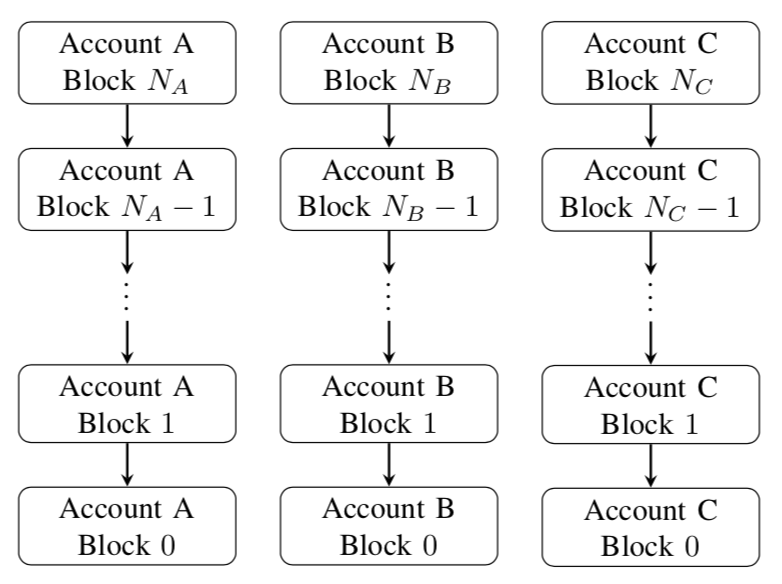
\includegraphics[scale=0.5]{images/RaiBlock_account_blockchain.png}
    \caption{Accounts with their corresponding block chains}
    \label{fig:rai-acc-chain}
\end{figure}

Making transactions from one account to another is done in two steps; the sender creates a send block on his account chain, and broadcasts it to the network. When broadcast, the amount is deducted from the sender's balance. The receiver then creates a receive block on his account chain in order to receive and thus update the receivers balance. A visualization of this can be seen in figure \ref{fig:rai-block-lattice}, where $S$ indicates the creation of send blocks and $R$ indicates the creation of receive blocks, which are signed by the owner of the corresponding account chain. The order of which the receive blocks are created does not matter as the sum is associative.

\begin{figure}[H]
    \centering
    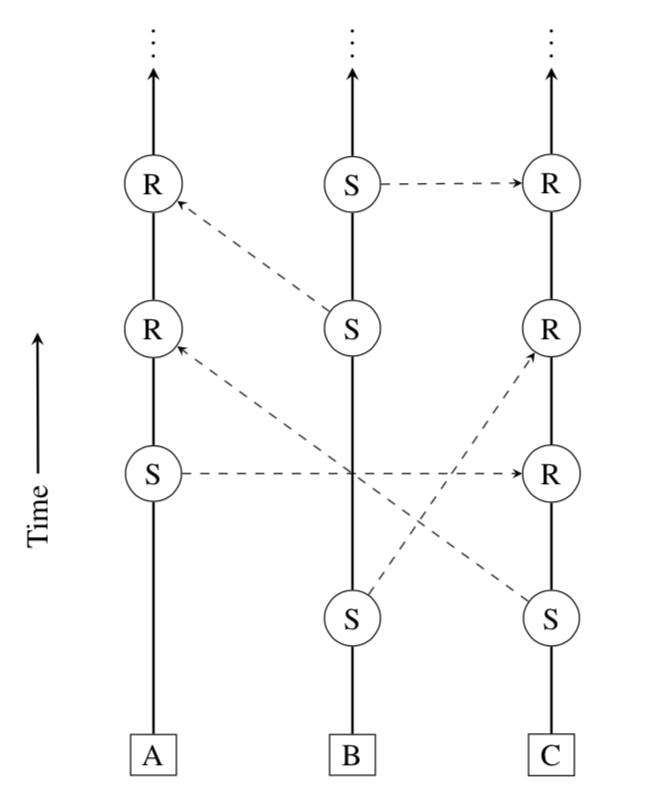
\includegraphics[scale=0.4]{images/RaiBlock_blocklattice.png}
    \caption{The block-lattice with send and receive blocks }
    \label{fig:rai-block-lattice}
\end{figure}

For maintaining the network, the aforementioned nodes validate transactions, when accounts make transactions, the nodes verify that the block does not already exist in the ledger, it is signed by the owner, that the previous block is the head of the account chain, the account chain has an open block and that the computed hash meets the Proof-of-Work threshold. The Proof-of-Work threshold in this system does not function as in Bitcoin, but as an anti-spam tool for issuing new blocks for an account.


If conflicting transactions, i.e., a fork on an account chain are found during the execution of the protocol, a vote is started in order to settle which transaction to keep. Each node has a weight, which is based on how much balance the accounts that have elected them as a representative has. Selecting a representative is first done when creating an \emph{open} block on the accounts chain, this representative can be themselves. The representative can be modified by creating a \emph{change} transaction. Each honest representative will always vote for the block that first came into their view.
The vote lasts for four voting periods, which lasts one minute in total and confirm the winning block based on:
\begin{align*}
    v(b_j) &= \sum_{i=1}^M w_i \mathbb{1}_{\hat{b_i} = b_j}\\
    b^* &= \underset{b_j}{arg max} \; v(b_j)
\end{align*}
With the block $b^*$ having the majority of votes, it will be retained in the node's account chain, the losing blocks are discarded. When a node replaces the loosing block with a winning block, it starts a new vote with a higher sequence number. Nodes \emph{only} vote when conflicting transactions are detected.

\subsection{Presented Attacks}
The RaiBlocks paper \cite{raiblocks} presents how it deals with \emph{Block Gap Synchronization}, \emph{Transaction Flooding}, \emph{Sybil Attack}, \emph{Penny-Spend Attack}, \emph{Precomputed PoW attack}, \emph{>50\% Attack}, and \emph{Bootstrap poisoning}. In this thesis a few of these attacks will be mentioned, as well as how the consensus deals with them.

\paragraph{Block Gap Synchronization}
Due to the possibility of brief network connectivity issues, a block may not be broadcast properly, which can lead to subsequent blocks not being received by the network. Due to this issue, if a node receives a block, which does not reference the previous block, the node can do one of two things; it can either ignore the block, since it could be a malicious block or it can request a resync with another node. If the node chooses to request a resync, the network traffic will increase, which can result in a \emph{Denial of Service (DoS)} if done in a maliciously way. To avoid this kind of malicious behaviour, the nodes will only do the resync, if it receives a certain amount of votes for a potentially malicious block. Otherwise, the node will consider the block to be garbage. 


\paragraph{Precomputed PoW Attack}
An owner can precompute a lot of sequential blocks with their PoW and then broadcasts them all at the same time to the network. This will flood the network with a lot of valid transactions, which the nodes need to process and echo to other nodes. This will result in a DoS attack. In \cite{raiblocks} this is still an open issue, but mentions they are looking into transaction rate-limiting and other techniques for dealing with it.

\paragraph{$>50\%$ Attack}
Compared to PoW systems where >50\% attack represents computing power. The consensus metric in RaiBlocks is the weighted voting system, as such the >50\% attack representing an adversary owning >50\% voting power. If an adversary gains this much power, they can cause the network to oscillate consensus rendering the system broken. Users with a high balance are incentivized to select honest nodes to maintain the network. Thus an adversary would need to convince high balance accounts to vote for him as a representative. Another proposed solution but not yet implemented suggestion is by doing block cementing, creating secure checkpoints which cannot be changed.


\subsection{Discussion}
While reading the paper, some concerns were discussed which will be presented in this section. It should be heavily noted that since the paper is very informal, the described concerns and attacks will also be informal or heavily relying on assumptions which will also be presented. It cannot be emphasized enough that a lack of a well-described formal model or evident reductions to well-known consensus protocols should be described in order to show security of their consensus mechanism.

% No incentive
The first raised issue with the protocol is, a node necessarily does not have an incentive to behave honestly. A node can have no stake, but in some way be popular enough s.t. other nodes pick it as a representative. At the point of having a majority of voting power this node can behave maliciously and destroy the network, as in the $>50\%$ attack described previously without any lost stake in the system, disregarding network resources while behaving honestly.\\

% PoW threshold?
RaiBlocks \cite{raiblocks} mentions a Proof-of-Work threshold in order to avoid flooding of transactions. In the appendix of \cite{raiblocks}, the threshold is mentioned to be static, which has no relation to the computational power within the already described system. Assuming that an average computer can do the Proof-of-Work with ease, a malicious adversary with a high amount of computational power would easily be able to flood the system with transactions. The appendix of \cite{raiblocks} also mentions an adaptive threshold, but shows no way of implementing it yet, and therefore it will not be further discussed. \\

% General network abstraction
Also inherently there is a lack of abstraction in \cite{raiblocks}. All of the cryptographic primitives are assumed to be known before-hand, thus not formalized or described in any way. Despite not using anything besides public-key cryptography, described in section \ref{sec:public-key}, as well as cryptographic hash functions, described in definition \ref{def:hash}, a short introduction of these should be in order for completeness. A model for the underlying network is also a problem, what attacks and what kinds of analysis is an adversary allowed to make throughout the execution of the protocol. In the previous chapters of Proof-of-Work \ref{cha:pow} and Proof-of-Stake \ref{cha:pos}, all of these primitives were abstracted into designated functionalities, so the focus could rely fully on the analysis of the consensus protocol.\\

From reading the RaiBlocks paper, two potential attacks came to mind, a \emph{Ping Pong Attack}, which is a DoS attack and a \emph{Receiver Fragmentation Attack}, which attacks the consensus of the receivers of a transaction.
% Presented attacks
%% Ping pong
\paragraph{Ping Pong Attack}
This attack is a way of generating a lot of noise within the network by continuously making nodes vote for consensus on a transaction thus creating a Denial-of-service attack. For this attack the following assumptions were made with regard to the RaiBlock protocol.
\begin{itemize}
    \item The representation distribution is stable.
    \item Messages are propagated through an underlying peer-to-peer protocol.
    \item Full voting representation.
    \item Adversary controls $1\%$ of the representation power.
\end{itemize}

The first is, users are not continuously changing their representative within the system, so assuming a stable representation distribution would seem like a reasonable assumption. The second assumes a underlying peer-to-peer network, where nodes are not fully connected but messages are propagated throughout the network in \emph{some} way, such that building a potential network graph would be possible. For simplicity of the attack full network representation is expected and that the adversary controls $1\%$ of the representation power.

\begin{enumerate}
    \item Network analysis: Keep introducing regular transactions to build a network graph on how communication is propagated. From this the adversary can create a flow graph of the network without creating conflicts.
    \item The adversary precomputes two conflicting transactions $m_1, m_2$, that reference the same previous transaction $m$.
    \item Introduce $m_1, m_2$, such that it fragments the nodes equally.
    \item Upon detecting the conflicting transaction nodes will issue votes.
    \begin{enumerate}
        \item The adversary can decide the winner of the nodes with his $1\%$ representation power. Always opting to replace the message a node saw first.
        \item Upon replacing a message a node will create a new vote, as described in the protocol. Which will repeat from a)
    \end{enumerate}
\end{enumerate}

The amount of conflicting messages are not limited to two, but an adversary can pick them depending on how many nodes that have a large share of representative weight to potentially increase the potential for a successful fragmentation. Assuming some network changes or general activity changes of the peers within the system, eventually the vote will skew towards one of the messages which will be retained, but the attack will still heavily flood the network with continuous votes. This attack also gets easier the more representative power an adversary possesses, as he would have more impact on the result of the vote, making the attack easier to execute.



%% Fragmentation attack
\paragraph{Receiver Fragmentation Attack}
This is an attack that can fragment the receivers account chain by attacking the voting consensus mechanism in RaiBlocks. For this attack the following assumptions were made with regard to the RaiBlocks protocol. 
\begin{itemize}
    \item The representation distribution is stable.
    \item Messages are sent point-to-point to each node maintaining the network, without package loss.
    \item Full voting representation.
    \item Adversary controls $1\%$ of the representation power. 
\end{itemize}

The first assumption is based on users not often changing representatives in the system, assuming the network is stable, this would seem like a reasonable assumption. The second assumption is simply due to not having described any underlying network of communications in \cite{raiblocks}, as such it may be a simplifying assumption but this will be extended to having an assumption of an underlying network later. The third assumption, full voting representation, is an extension of the point-to-point, as all representatives have the messages and all also get the conflict message. Last assumption is that the adversary has a little control over the network in terms of influencing votes. The attack is carried out in the following way.

\begin{enumerate}
    \item The adversary forks his account-chain and broadcasts transaction $m$ to one half of the network $H$ and $m'$ to the other half $H'$, based on their voting power.
    \item The adversary then sends $m$ to receiver $R$ and $m'$ to receiver $R'$.
    \item The malicious representative starts a vote before other conflicts have been found, thus controlling the vote. After the voting has finished the half $H$ has voted on $m$ and $H'$ voted on $m'$. Thus the malicious representative can have the deciding vote, and fragment the final result by sending that $m$ is the winner to $H$ and $m'$ is the winner to $H'$.
\end{enumerate}

Though the assumption in the stated attack is point-to-point communication during broadcasts, it can instead be extended to an underlying peer-to-peer protocol, for broadcasting messages, where we assume a fairly stable network.

\begin{enumerate}
    \item Network analysis: Keep introducing regular transactions to build a network graph on how communication is propagated. From this the adversary can create a flow graph of the network without creating conflicts. 
    \item The adversary then introduces the 2 conflicting transactions $m'$ and $m$, to the network in such a way that the network is split in half.
    \item The adversary then again creates the conflicting vote, and fragments the network as in the previous stated attack.
\end{enumerate}

It should be noted that in our assumptions the adversary only controls 1\% of the voting power, with increased power the chance for success especially in the case with an underlying peer-to-peer system increases.

By carrying out this attack, the adversary fragments the receivers account across the network and creates inconsistent views among the nodes, this can continuously be done such that the system is fully inconsistent, and thus unusable.


% IOTA - 
\section{IOTA}
IOTA is not based on the popular blockchain structure, but it is based on a structure called the tangle. The tangle is a new way to structure a ledger system and it is based on \emph{directed acyclic graphs}. The tangle is developed to address some of the drawbacks known from the blockchain technology, e.g. micropayments being too expensive due to the transaction fee. The Bitcoin blockchain structure also consists of two distinct types of actors within the system, namely parties who issue transactions and parties who validate transactions. This can lead to the parties having different goals, as the miners are interested in raising fees such that they get as much money rewarded as possible, while peers wanting to make transactions want the transactions to be as cheap as possible.\\


% Design
The IOTA network consists of nodes, which can both issue a transaction and validate transactions. The general idea is, when nodes want to issue a transaction it will have to approve other transactions, i.e., checking whether or not the transactions are conflicting before directly or indirectly approving them. In particular, if a node wants to issue a transaction, it chooses two other transactions which it is going to approve. When two approving transactions are found, the node will issue a valid transaction, which is done by computing a Proof-of-Work as in the Bitcoin protocol. This Proof-of-Work only exists to mitigate spamming the network with transactions, like in the RaiBlocks system. Therefore, issuing transactions are also contributing to the security of the network by further confirming previously made transactions.\\

Since the network is asynchronous, nodes do not necessarily see the same set of transactions. This leads to the tangle may hold conflicting transactions, \cite{tangle} notes that the tangle is allowed to hold them, but the protocol must agree on which of the conflicting transactions are valid, as such, the consensus protocol has to agree on which transactions will be orphaned. For this a so-called \emph{tip-selection algorithm} is used to choose which transactions to validate, as such, much of the consensus is based on how these tips are selected.\\


An illustration of a tangle is shown in figure \ref{fig:iota-tangle}, which originates from the genesis block, in which the site $G$, a transaction located on the tangle, approves the genesis block. Any site located after these two sites will always reference two previous sites. A site has a corresponding weight and a score. The weight is based on the amount of work done in its Proof-of-Work, and the score is the sum of own weights of all the sites directly or indirectly approved by a given site plus its own weight. In the example provided in figure \ref{fig:iota-tangle}, $A$ has an own weight $A_w = 1$ and the score is $A_{score}=9$ as $A$ approves sites $G,F,D$ and $B$.
\begin{align*}
    A_{score} = G_{w} + F_{w} + D_{w} + B_{w} + A_{w} = 1 + 3 + 1 + 3 + 1 = 9
\end{align*}

\begin{figure}[H]
    \centering
    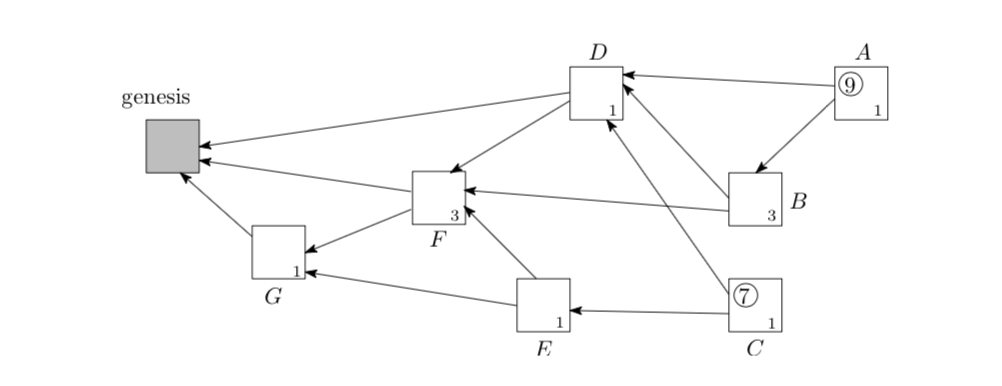
\includegraphics[width=\linewidth]{images/iota-score.png}
    \caption{Tangle with transactions and their corresponding score and own weight.}
    \label{fig:iota-tangle}
\end{figure}

The notion of cumulative weight is introduced as the site's own weight plus the sum of all transaction that directly or indirectly approve this site. Intuitively, this is viewed as how much cumulative work that has been done to approve this site. Figure \ref{fig:iota-transaction} illustrates this, the cumulative weight is in bold of each site. With the introduction of a new site $X$ with weight $3$, it increments the cumulative weight of all previous sites by $3$, as it directly or indirectly approves all other sites. The cumulative weight is the metric used to know when transactions are considered validated within the system, such that a receiver can consider the transaction valid once it has enough cumulative weight.

\begin{figure}[H]
    \centering
    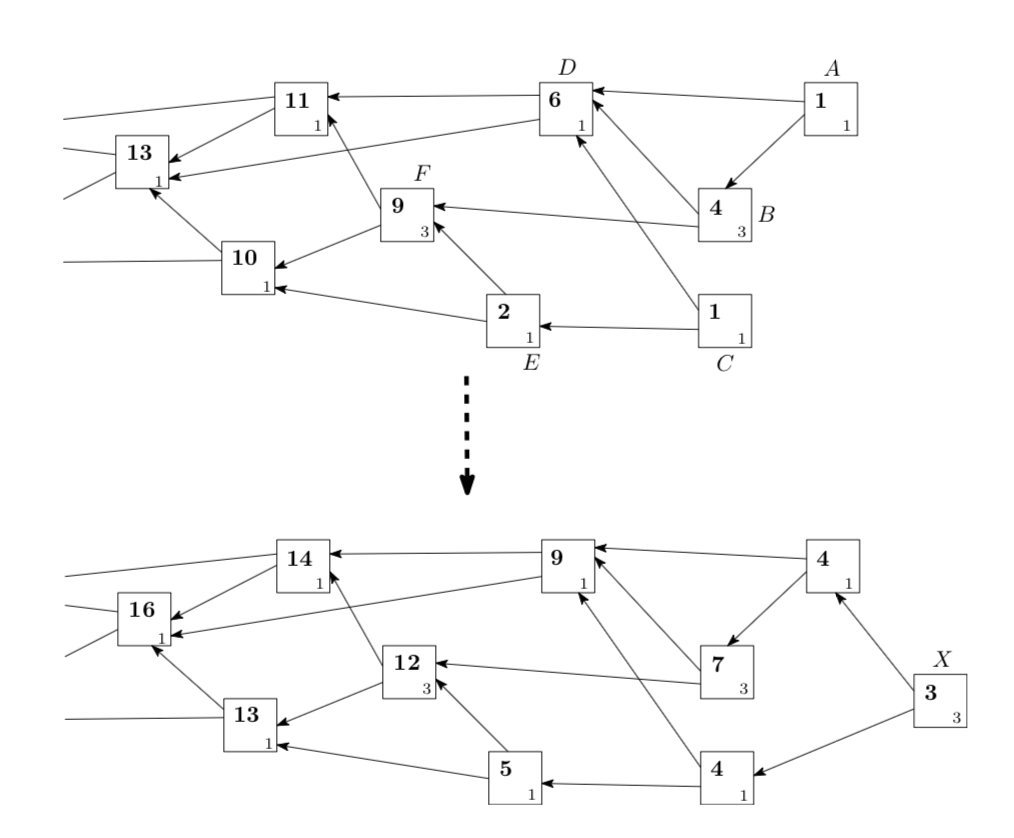
\includegraphics[width=\linewidth]{images/iota-cumulative-weight.png}
    \caption{Tangle with transactions and their corresponding cumulative (bold) and own weight.}
    \label{fig:iota-transaction}
\end{figure}


\subsection{Analysis}

\cite{tangle} does not provide any formal security model, but do present a few arguments of security and consistency that will be covered in this section.

For the analysis of the protocol, a couple of simplifying assumptions are made in \cite{tangle} in order to simplify the analysis.
\begin{itemize}
    \item $L(t)$ is defined as the total number of tips at a given time $t$. It is a stochastic process, which should remain stable, i.e., fluctuate around a constant and will not escape to infinity. The total number of tips is concentrated around a number $L_0 > 0$.
    \item Transactions are roughly independent, s.t., they can be modeled by a Poisson point process.
    \item The Poisson process rate, $\lambda$, is constant in time.
    \item All devices have approximately the same computing power, and simply picks two random valid tips and approves them.
    \item When a node wants to issue a transaction, it does not observe the actual state of the tangle, but instead the tangle $h$ time units ago. This means a node will only be able to view the full tangle at time $t$ at time $t+h$, in which the transaction also becomes visible to other nodes.
    \item Without loss of generality it is assumed that all weights of sites is 1, thus the cumulative weight is the sum of all direct or indirectly approving sites plus 1.
\end{itemize}

% Stability - show that L(t) is stable around L_0 = 2lambda h
To formalize $L_0$, it is defined to be a function of $\lambda$ and $h$. At time $t$ there is $\lambda h$ hidden tips and $r$ revealed tips. As such the total number of tips is $L_0 = r + \lambda h$. Given a transactions is made, selecting a tip randomly as assumed, the probability of selecting a tip is $\frac{r}{r+\lambda h}$. As the number of tips remains roughly constant in time
\begin{equation*}
    \frac{2r}{r+\lambda h} = 1 \implies r = \lambda h \implies L_0 = 2\lambda h
\end{equation*}

This can be further generalized for a transaction to reference $k$ transactions instead of $2$ with $L_0^{(k)} = \frac{k \lambda h}{k-1}$.

For the analysis two cases are considered, a low-load, i.e., $L_0$ is low, and a high-load, i.e., $L_0$ is high, as illustrated in figure \ref{fig:iota-low-high-load}:
\begin{itemize}
    \item \textbf{Low-load: } The case where the number of tips is small, and frequently becomes 1. Given the low amount of transactions it may happen that several different transactions approve the same tip. For this, it has to be assumed that \emph{an adversary does not inflate the number of tips}. See the top tangle in figure \ref{fig:iota-low-high-load} for an illustration. 
    \item \textbf{High-load: } The case where the number of tips is large. This can be due to a large flow of transactions, in combination with computational delays and network latency, making it possible for multiple transactions to approve the same tip. See the bottom tangle in figure \ref{fig:iota-low-high-load} for an illustration. 
\end{itemize}

\begin{figure}[H]
    \centering
    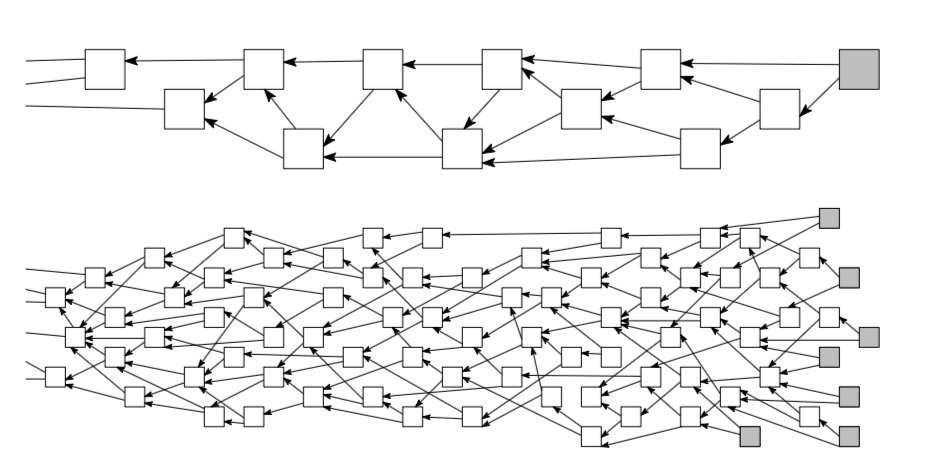
\includegraphics[width=\linewidth]{images/iota-low-high-load.png}
    \caption{Top: Tangle with low load. Bottom: Tangle with high load}
    \label{fig:iota-low-high-load}
\end{figure}

It is trivial to see that the first approval of a tip in the low-load case given $L_0$ frequently becomes $1$, this means as soon as a transaction is propagated to the network, it will be selected as a tip for the next transaction. Thus a tip gets approved for the first time in $\Theta(\lambda^{-1})$ time units, where $\lambda$ is the rate of incoming flow of transactions.\\

The high-load case, which is the case where $L_0$ is large. \cite{tangle} assumes that the Poisson flow of approvals to different tips is $\frac{2\lambda}{L_0}$, which gives that the expected time for a tip to get its first approval is 
\begin{equation}
    \frac{L_{0}}{2\lambda} = \frac{2\lambda h}{2\lambda} \approx \Theta(h)
\end{equation}
It should be noted, if a tip $t$ is not approved by $\Theta(h)$ time, then it would be a good strategy to promote it by creating an empty transaction, which approves $t$ together with a newer tip $t'$. This strategy improves the probability of $t$ being approved, due to $t'$ being newer and more preferable to choose, and thereby making the new empty tip more preferable to approve. \\


% Weight growth - how fast?
In order to confirm that transactions have been included in the tangle, a metric for when they are fully approved to be part of it must be defined. For this the cumulative weight is used in order to confirm transactions with higher level of confidence. Thus showing the speed of which the cumulative weight of a site needs to be considered. Here the two extreme cases; the low-load case and the high-load case are considered. 

The low-load case is trivial, as explained earlier, given a new transaction, it will always approve the previous transaction, the following transactions will thus indirectly approve that transaction. Thus the cumulative weight will grow by $\lambda$, due to the simplification that all weights are $1$.

In the high-load case, given that a transaction already has a high cumulative weight in the tangle, each new transaction will indirectly verify this transaction and thus always have an increasing weight of $\lambda$. Thus showing how fast it grows until it achieves a high cumulative weight is required. Let $H(t)$ be the the cumulative weight for a transaction at time $t$, which starts counting when the transaction is available to the network, i.e., $h$ time units after creation. Let $K(t)$ be the expected number of tips that approve the transaction at time $t$. Thus the probability for a transaction approving at least one of those tips that directly or indirectly approves a given transaction is 
\begin{equation}
\label{eq:iota-our-tip-selected}
    1- \left(1- \frac{K(t-h)}{L_0}\right)^2 = \frac{K(t-h)}{L_0}\left(2-\frac{K(t-h)}{L_0}\right)
\end{equation}

Utilizing this probability, the expected cumulative weight will at time $t+\delta$ be

\begin{equation}
\label{eq:iota-expected-cumu-weight}
    H(t+ \delta) = H(t) + \lambda \delta \frac{K(t-h)}{L_0}\left(2-\frac{K(t-h)}{L_0}\right) + o(\delta)
\end{equation}

In equation \ref{eq:iota-expected-cumu-weight}, the second term of the equation is the probability from \ref{eq:iota-our-tip-selected} with respect to the flow of incoming transfer over time units $\delta$. The last term of the equation is the asymptotic \emph{little-o} with regard to $\delta$. From equation \ref{eq:iota-expected-cumu-weight}, the derivative can be deduced.

\begin{equation}
\label{eq:iota-derivative}
    \frac{dH(t)}{dt} = \lambda \frac{K(t-h)}{L_0}\left(2-\frac{K(t-h)}{L_0}\right)
\end{equation}


For utilizing equation \ref{eq:iota-derivative}, $K(t)$ also needs to be calculated. This is not as simple since a tip at time $t-h$ is not necessarily a tip at time $t$. But as noted earlier, the typical number of tips is $2\lambda h$ and during an interval of length $h$, $\lambda h$ new tips will replace previous ones, as such the probability of a tip at time $t-h$ remains a tip at time $t$ is approximately $1/2$. To advance the calculation of $K(t)$ two sets are defined, a set $A$ containing all the $K(t-h)/2$ tips that are not approved by time $t$, and another set $B$ containing all the $K(t-h)/2$ tips that are approved by time $t$. With regard to these two sets, two probabilities are defined $p_1$ and $p_2$. The second probability $p_2$ is that both the approved tips are contained in the set $B$.

\begin{equation*}
    p_2 = \left( \frac{K(t-h)}{2L_0} \right)^2
\end{equation*}

The first probability $p_1$ is similar to $p_2$, though it is extended with twice the probability that the first tip is contained in $B$ and the second tip is not contained in $A \cup B$. 

\begin{equation*}
    p_1 = \left( \frac{K(t-h)}{2L_0} \right)^2 + 2 \cdot \frac{K(t-h)}{L_0} \left( 1-\frac{K(t-h)}{L_0} \right)
\end{equation*}

By these two probabilities and the incoming transaction flow $\lambda$, the derivative can be found for $K(t)$.


\begin{equation}
\label{eq:iota-derivative-k}
\frac{dK(t)}{dt} = (p_1 - p_2)\lambda = \lambda\frac{K(t-h)}{L_0} \left( 1-\frac{K(t-h)}{L_0} \right)
\end{equation}

Since it is a difficult task to solve equation \ref{eq:iota-derivative-k}, \cite{tangle} makes some simplifying assumptions. First, they note that when $K(t)$ reaches level $\varepsilon L_0$ for $\varepsilon > 0$, which denotes the adaption period has ended, $K(t)$ quickly grows to $(1-\varepsilon)L_0$. Furthermore, when $K(t)$ is small with respect to $L_0$, the last factor of equation \ref{eq:iota-derivative-k} becomes a constant very close to 1, and can therefore be dropped. By utilizing that $\frac{\lambda h}{L_0} = \frac{1}{2}$, equation \ref{eq:iota-derivative-k} can be rewritten.

\begin{equation}
\label{eq:iota-derivative-k-new}
    \frac{dK(t)}{dt}\approx \frac{1}{2h} K(t-h)
\end{equation}

Here it should be noted that $K(0)$ is bounded to 1. \cite{tangle} wants to find a solution for $K(t)$ being on form $e^{c \frac{t}{h}}$. The desired form of $K(t)$ will be substituted into \ref{eq:iota-derivative-k-new} and by using the derivative quotient rule $\frac{de^{b \cdot x}}{dx} = b \cdot e^{b \cdot x}$ with respect to $x$, the updated equation of \ref{eq:iota-derivative-k-new} is on the following form.

\begin{equation*}
    \frac{c}{h} \cdot e^{c \frac{t}{h}} \approx \frac{1}{2h} \cdot e^{c \frac{t}{h} - c}.
\end{equation*}


To estimate the time, where $K(t)$ reaches level $\varepsilon L_0$, \cite{tangle} makes an approximate solution for $K(t)$ by making use of the \emph{Lambert W-function}, which is also known as the product logarithm, in the place of $c$: $K(t) = e^{W(\frac{1}{2}) \frac{t}{h}} \approx e^{0.352 \cdot \frac{t}{h}}$. By taking the logarithm, it can be estimated when the end of the adaption period is reached.

\begin{equation*}
    t_0 \approx \frac{h}{W(\frac{1}{2})} \cdot (\ln L_0 - \ln \varepsilon^{-1}) \lesssim 2.84 \cdot h\cdot \ln L_0
\end{equation*}

Now that $K(t)$ has been estimated, the focus can return to $H(t)$ and its derivative, where the following holds during the adaption period.

\begin{align*}
    \frac{dH(t)}{dt} \approx \frac{2\lambda}{L_0}
    \approx \frac{1}{h \cdot e^{W(\frac{1}{2})}} e^{W(\frac{1}{2})\frac{t}{h}}
    \approx \frac{W(\frac{1}{2})}{h} e^{W(\frac{1}{2})\frac{t}{h}}
\end{align*}

From this derivative during the adaption period, the expected cumulative weight at time $t$ for a given transaction can be estimated to $H(t) \approx exp(W(\frac{1}{2})\frac{t}{h})\approx exp(0.352 \cdot \frac{t}{h})$.


A graph showing how the cumulative weight grows in the high-load case is seen in figure \ref{fig:iota-cumulative-weight}. It shows that when a transaction gets introduced to the system, it will first enter an adaption period which has exponential growth until it is deep enough in the tangle, such that any new transaction indirectly validates it. After the adaption period, its cumulative weight increases by the speed transactions are introduced to the system, $\lambda$.

\begin{figure}[H]
    \centering
    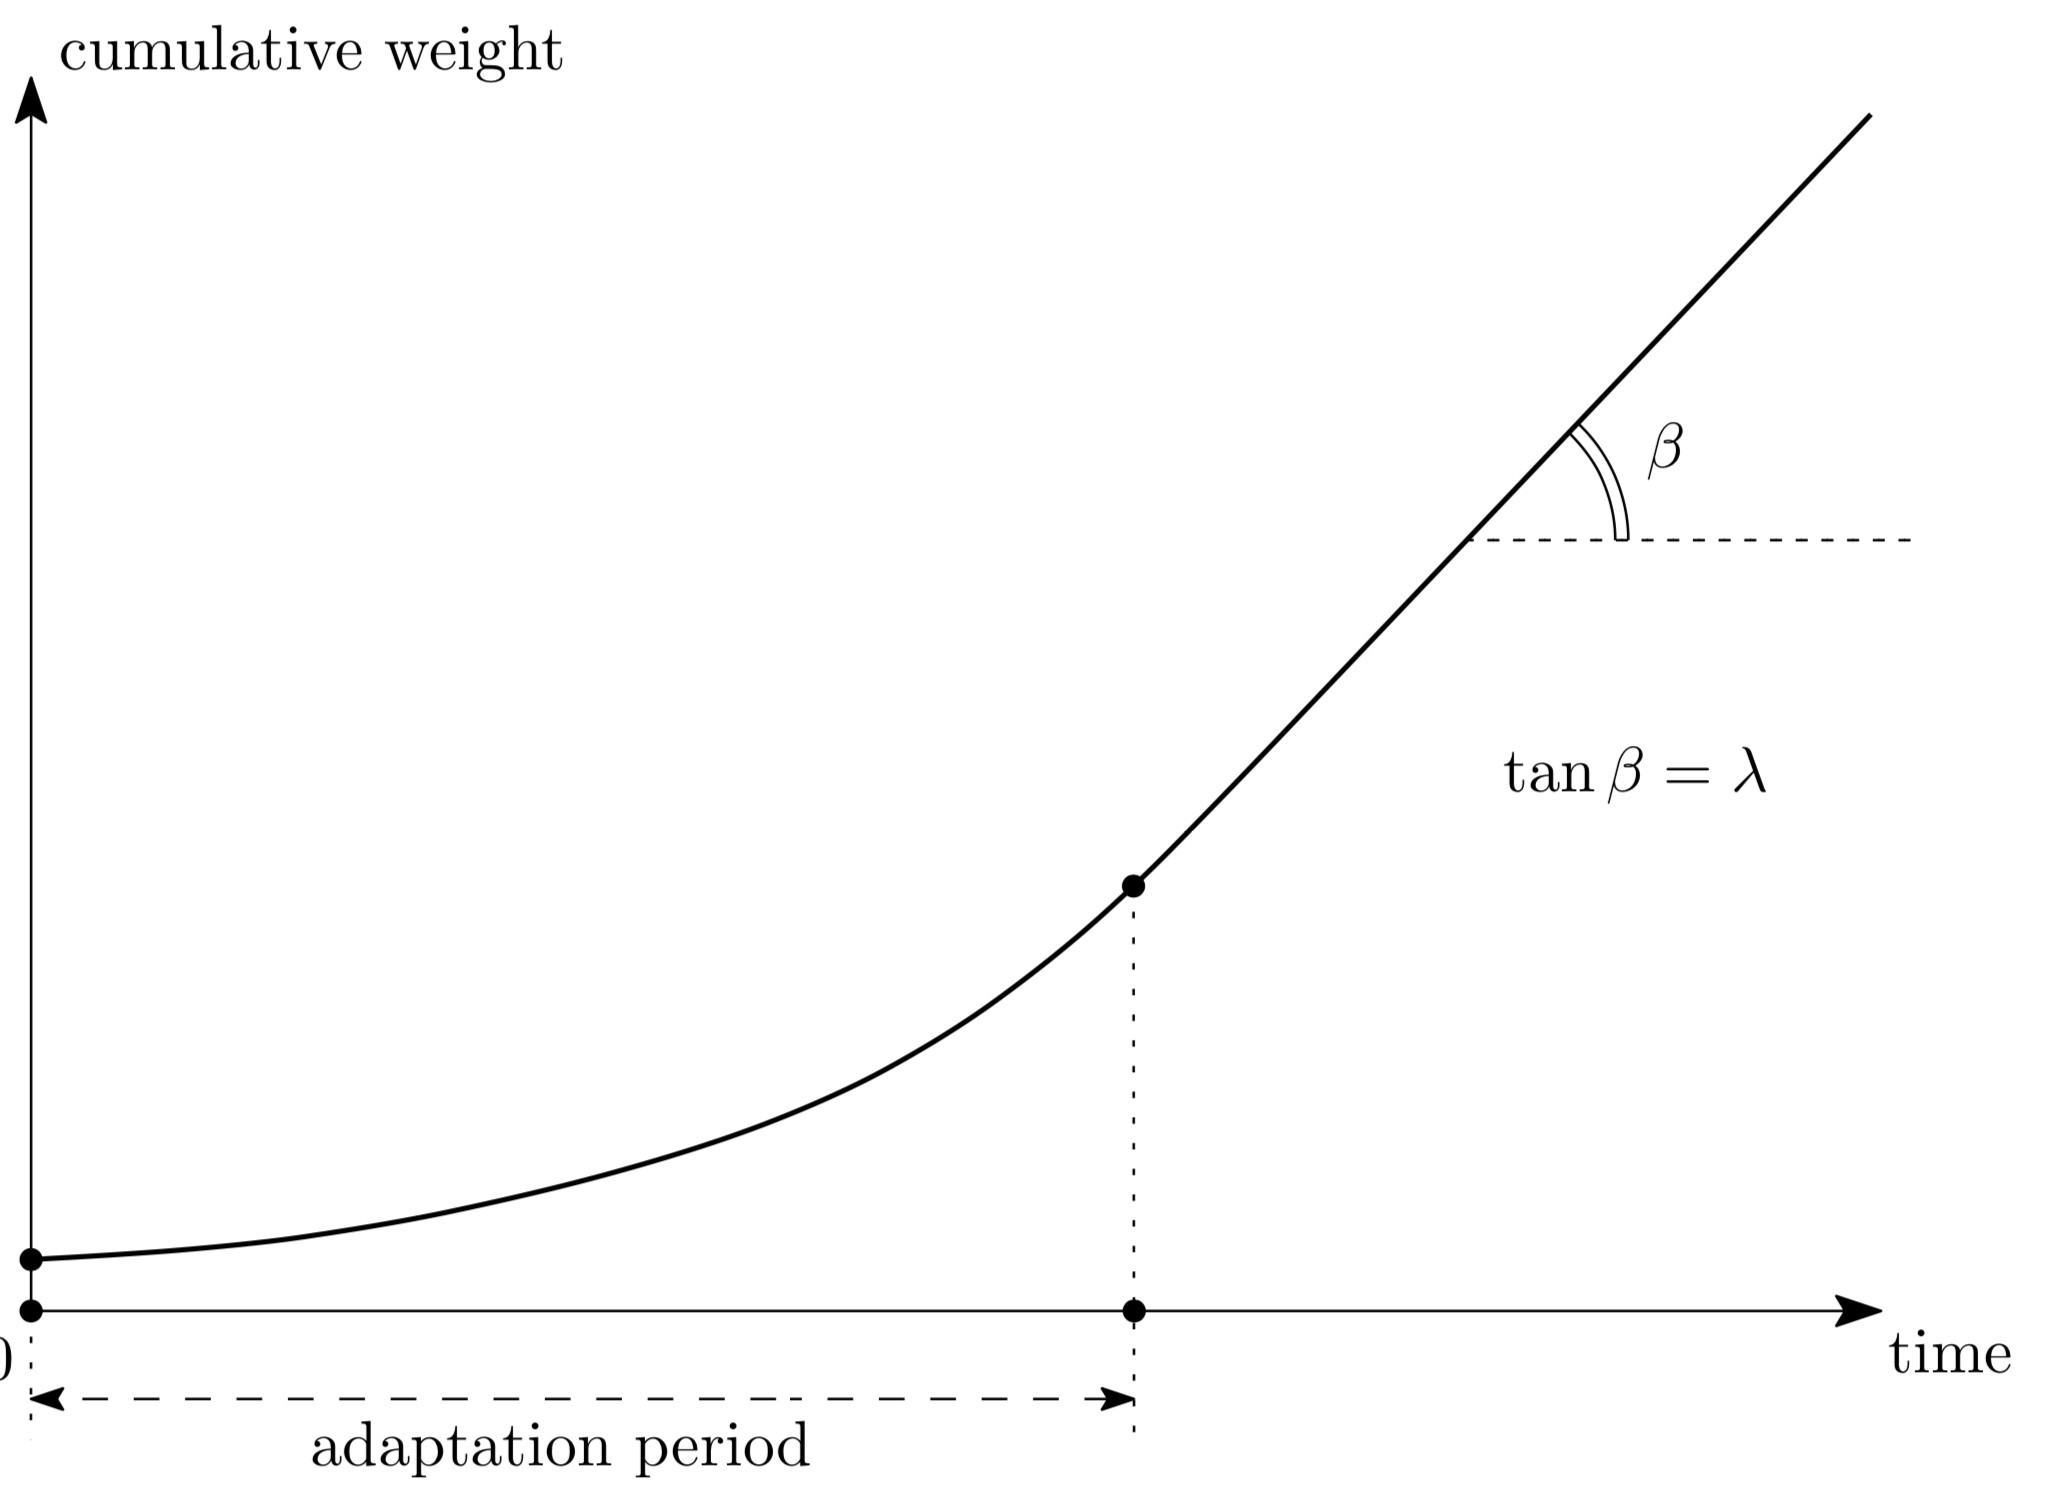
\includegraphics[scale=0.3]{images/iota-cumulative-weight-graph.png}
    \caption{Cumulative weight in the high-load case}
    \label{fig:iota-cumulative-weight}
\end{figure}

% Tip selection
It should be noted that a random tip selection strategy is not very good, since the adversary can potentially inflate the number of tips, which makes his transactions much more likely to be picked. Therefor an alternative tip selection algorithm called the \emph{Markov Chain Monte Carlo algorithm} for selecting tips will be described in the \emph{parasite chain attack} as a more practical tip selection algorithm.

% Attacks
\subsection{Attacks}
\cite{tangle} presents a couple of attacks against their protocol, namely a \emph{Double spending attack}, \emph{parasite chain} and a \emph{splitting attack}.

\paragraph{Double spending attack}
\begin{enumerate}
    \item The adversary presents a transaction $tx$ and awaits a sufficiently large weight for the transaction to be accepted.
    \item The adversary tries to double spend by presenting a conflicting transaction $tx'$.
    \item The adversary uses its computing power to issue small transactions to approve the double spend, or if weights may be different from 1, issue the transaction with a large own weight.
    \item The adversary hopes that the dishonest subtangle outpaces the honest subtangle, in which the transaction $tx$ is orphaned effectively double-spending.
\end{enumerate}

In \cite{tangle}, $W^{(n)}$ denotes the time it takes to compute a valid transaction through Proof-of-Work of weight $3^n$ and $\mu$ denotes the computational power of the adversary. It is assumed that $W^{(n)}$ is an exponentially distributed random variable with parameter $\mu 3^{-n}$ and $w_0$, the weight when a transaction is accepted, happens at $t_0$ time units after the original transaction. It is assumed that the weight grows at a linear speed $\lambda w$, in which $\lambda$ is the rate of transactions, and $w$ is the mean weight of a generic transaction. Thus $w_1 = \lambda w t_0$ will be the typical weight of the honest branch at that time. If an adversary finds nonce such that $3^{n_0} \geq w_1$, where $n_0 = \lceil \frac{ln w_1}{ln 3} \rceil$, the attack succeeds. The probability of such an event occurring is:

\begin{equation*}
    Pr[W^{(n_0)} < t_0] = 1 - e^{-t_0 \mu 3^{-n_0}} \approx 1 - e^{-t_0 \mu w_1^{-1}} \approx \frac{t_0 \mu}{w_1}
\end{equation*}

In which the approximation holds when $\frac{t_0 \mu}{w_1}$ is small. Even if the attack does not succeed, the adversary may proceed to try finding a larger weight $3^n$ s.t. $n > n_0$, in which the legitimate branch has a smaller weight than $3^n$. The probability of this can be computed as:

\begin{align*}
    Pr[\lambda w W^{(n)} < 3^n] &= 1 - e^{-\mu 3^{-n_0} \cdot (3^{n_0}/\lambda w)}\\
    &= 1 - e^{-\mu / \lambda w} \\
    &\approx \frac{\mu}{\lambda w} \\
\end{align*}

Now despite $\frac{\mu}{\lambda w}$ typically being a small number, it is not negligible, thus countermeasures are required. By having the flexibility to change the weights, the ability to easily compute spam transactions can be reduced. \cite{tangle} mentions that capping the value of a single transaction to a lower weight is ideal. For simplicity to analyze the protocol, the weight of a transaction is capped to $1$ and estimated if such an attack would succeed. Instead of generating a single large transaction, one double-spending transaction is created while the adversary will generate nonsense transactions referencing the double-spending transaction, to boost the weight of the double-spending transaction.\\


 \cite{tangle} denotes $G_1, G_2, ...$ as i.i.d exponential random variables with parameter $\mu$, such that the expected value is $1/\mu$, and defines $V_k = \mu G_k$ with parameter $1$, where $k \geq 1$. The moment generating function of a exponential distribution with parameter $1$ is defined as $M(\theta) = (1 - \theta)^{-1}$ \cite{Moment-generating-function}. Furthermore, $\alpha \in (0,1)$ and $\varphi(\alpha) = \ln \alpha + \alpha - 1$ as the Legendre transformation of ln $M(-\theta)$. Stated in \cite{tangle} the following equation is known from the field of \emph{Large Deviation Principles}:

\begin{equation}
\label{eq:tangle-ldp}
    Pr[\sum_{k=1}^n V_k \leq \alpha n] \approx e^{-n \varphi(\alpha)}
\end{equation}

As the adversary has less computing power than the honest tangle, it is assumed that $\frac{\mu t_0}{w_0} < 1$. If the adversary wants to succeed with the double spending attack, he needs to generate at least $w_0$ transactions with own weight $m$ at time $t_0$. From equation \ref{eq:tangle-ldp}, the probability the double-spending $\frac{w_0}{m}$ transaction has more cumulative weight at $t_0$ can be calculated as being:

\begin{align}
\label{eq:tangle-double-spend-cumu}
    Pr[\sum_{k=1}^{w_0 / m} G_k < t_0] &= Pr[\sum_{k=1}^{w_0} V_k < w_0 \cdot \frac{\mu t_0}{w_0}]\\
    &\approx e^{- w_0 \varphi(\frac{\mu t_0}{w_0})}
\end{align}

From the result in equation \ref{eq:tangle-double-spend-cumu}, it follows that for the probability to be small $\frac{w_0}{m}$ needs to be large, implying that $\varphi(\frac{\mu t_0}{w_0})$ cannot be small.

Thus that at any time $t \leq t_0$, the weight of the honest transaction is $w_0 + \lambda(t - t_0)$, which is due to the assumption that the adaption period is over. This means the cumulative weight grows with speed $\lambda$. 

\begin{equation*}
    e^{-(w_0 + \lambda(t-t_0)) \varphi(\frac{\mu t}{w_0 + \lambda(t-t_0)})}
\end{equation*}

Thereby, $\frac{\mu t_0}{w_0} \leq \frac{\mu}{\lambda}$ since the cumulative weight grows with speed less than $\lambda$, the chance of making a double spend is:

\begin{equation}
\label{eq: tangle-security}
    e^{-w_0 \varphi(\max(\frac{\mu t_0}{w_0}, \frac{\mu}{\lambda}))}
\end{equation}

\cite{tangle} provides examples of the result in the equation \ref{eq: tangle-security}. Given $\mu = 2, \lambda = 3$, the probability of double spend is calculated to be approximately $0.29$, and if $\mu = 1, \lambda = 3$ then it would be approximately $0.00001135$, showing that the probability of a successful double spend drops exponentially depending on the adversarial computation power. This also shows that in order to provide any security within the system $\lambda > \mu$, i.e., honest peers generate more transactions than malicious peers.

%% Parasite chain
\paragraph{Parasite chain} 
This attack is based on the adversary to create a subtangle in secrecy. For this secret subtangle, or parasite chain, to gain a higher score, it will sometimes refer to the main tangle. By doing this, the tips on the parasite chain will have a score containing the sum of all own weights in the main tangle, but also the sum of all weights in the parasite chain, where the score of the honest tips will only contain the sum of all own weights in the main tangle. When the adversary wants to carry out the attack, he has the possibility to artificially increase his tip count by broadcasting multiple new transactions, which will approve earlier issued transactions on the parasite chain. Now, the adversary will have an advantage when a simplistic tip selection algorithm is utilized.
The attack is illustrated in figure \ref{fig:tangle-parasite}.

\begin{figure}[H]
    \centering
    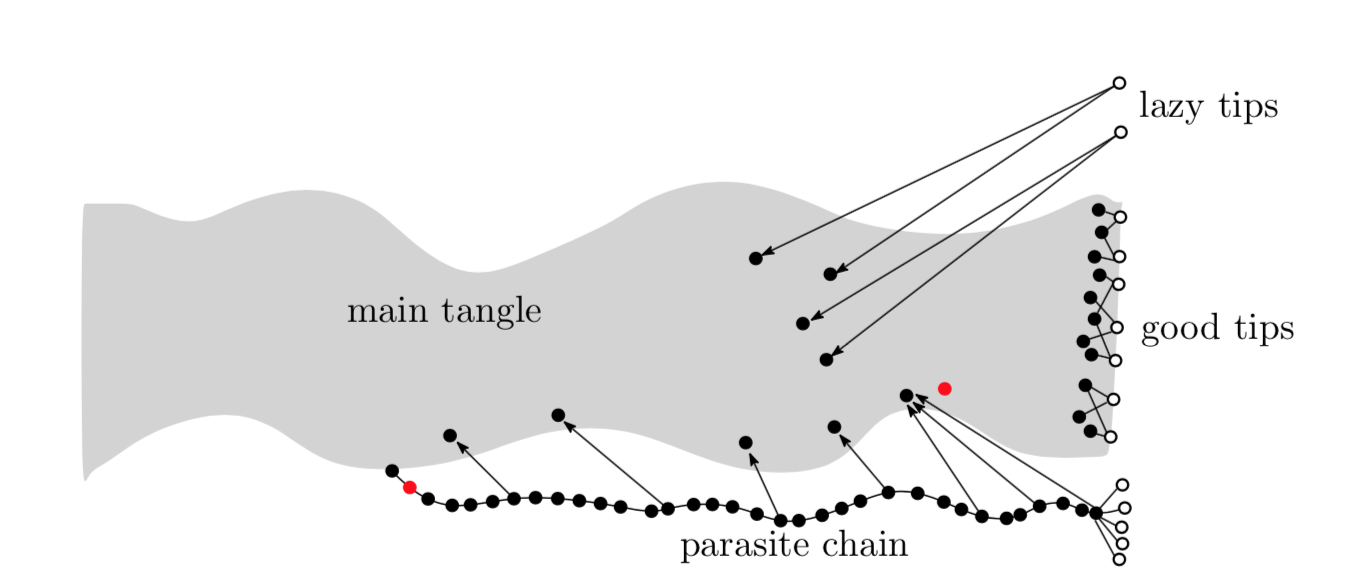
\includegraphics[width=\linewidth]{images/tangle-parasite-chain.png}
    \caption{Parasite chain attack}
    \label{fig:tangle-parasite}
\end{figure}


To deal with this kind of attack, \cite{tangle} presents a new tip selection algorithm, which is based on the \emph{Markov Chain Monte Carlo} algorithm and the fact that, the honest main tangle should have more hashing power than the parasite chain. Thereby, the honest parties will be able to create transactions such that, they will have a larger increase in cumulative weight than the transactions created by the adversary.

Intuitively, the new tip selection algorithm works by placing random walkers on the sites of the main tangle and let them walk towards the tips. Those tips the random walkers end up at are candidates for approval. More specifically, the algorithm from \cite{tangle} works in the following way:
\begin{enumerate}
    \item Consider all sites in the interval $[W,2W]$ from the tips. $W$ should be large such that a random walker will placed deep in the network and would not get to a tip immediately.
    \item $N$ particles will independently be placed on sites in the aforementioned interval. There are placed multiple random walkers for security, i.e., if a random walker is walking onto the parasite chain, which is supposed to be long, then it will spend some time before arriving at a tip, and then the random walkers at the main tangle should arrive at some honest tips before.
    \item The random walkers conduct independent discrete-time random walks towards the tips, i.e., they can only walk from one site to another if the latter site approves the former site.
    \item The two random walkers that first arrives at the tip set will indicate the two tips, which will be approved. \cite{tangle} notes, that a modification to this rule will be wise, such that if a random walker arrives at a tip too fast, then it will be discarded due to high probability of that tip being a \emph{lazy tip}, defined later.
    \item If a site $y$ approves $x$, denoted $y \rightsquigarrow x$, the transition probability $P_{xy}$ will be proportional to $e^{-\alpha (\mathcal{H}_x - \mathcal{H}_y)}$, where $\alpha > 0$ is a parameter to be chosen and $\mathcal{H}_x$ denotes the cumulative weight for $x$, such that
    \begin{equation}
    \label{eq:mcmc-transition-probabilities}
        P_{xy} = e^{-\alpha (\mathcal{H}_x - \mathcal{H}_y)} \left(\sum_{z:z\rightsquigarrow x} e^{-\alpha(\mathcal{H}_x - \mathcal{H}_z)}\right)^{-1}
    \end{equation}
\end{enumerate}

Checking that the algorithm works as intended, \cite{tangle} considers two cases. The first case considers the \emph{lazy tips} and the second case considers an alternate style of attack. In the first case, a lazy tip will approve some older sites such that it avoids doing verification work. Though avoid doing the verification work is not beneficial in this setting, since it is not probable the lazy tip will be selected. This is due to the difference between cumulative weights would be very large and $P_{xy}$ would be small. In the second case, an alternate attack is carried out in the following way:
\begin{enumerate}
    \item The adversary secretly creates a parasite chain. The parasite chain contains a transaction, which empties the adversaries account balance to another account, which he also controls. This transaction can be seen in figure \ref{fig:tangle-parasite} as the red dot located in the parasite chain. 
    \item The adversary then creates a transaction on the main tangle, which is illustrated as the red dot located on the main tangle in figure \ref{fig:tangle-parasite}. When it has been located on the main tangle, the adversary waits for it to be accepted. 
    \item While creating the parasite chain, the adversary makes sure that it once in a while refers some sites on the main tangle. Though it should be noted, that the parasite chain cannot refer the main tangle after the transaction done in step 2 is accepted, and thereby the cumulative weight cannot be large in the parasite chain.
    \item When the adversary wants to carry out the attack, he will artificially increase his tip count by broadcasting multiple new transactions.
\end{enumerate}
By the same reasoning as in the first case, this alternate attack will not work due to the sites on the parasite chain having smaller cumulative weight than the sites on the main tangle, and therefore the sites on the parasite chain will not be chosen with high probability by a random walker.  \\

\cite{tangle} remarks, it is very simple to calculate the exit probability distribution, when a random walk always moves towards the tips, which is not a wanted feature. Therefore, \cite{tangle} modifies their approach, such that on each step the random walker takes, there is a possibility of $1/3$ for it to backtrack, and thereby moving one step away from the tips. The random walker will still quickly arrive at the tips and furthermore, it would be more difficult to calculate the exit probability distribution. It could be considered why the parties in the network will be likely to follow this modified approach. According to \cite{tangle}, one of the reasons the parties of the network will follow this approach, is due to the assumption that at least a good portion of the parties will follow the chosen tip selection algorithm. Another reason is due to the delays, respectively network and computational, which cause the algorithm to rather work with a past snapshot of the tangle with respect to when a transaction is issued. As stated in \cite{tangle} it could be beneficial to place the snapshot further in the past, due to the risk of a party acting \emph{selfishly}, i.e. tries to maximize the chances of its transaction to be approved. 

Due to the assumption that a good portion of the parties follow the approach, the \emph{Markov Chain Monte Carlo} algorithm will define a probability distribution on the set of tips. A selfish party will try to select the tips placed at the maximum of the distribution, which will make its transaction more likely to be approved. Though, if multiple parties are acting selfishly, then they would not gain much, since they all approve the same tips, which leads to their transactions competing for approvals. Due to the tip selection algorithm working with a past snapshot, the selfish parties will not see the cumulative weight increase immediately, since the random walker first finds a former tip with respect to the past snapshot and then the random walker continues towards the tips of the current tangle. This means the probability distribution for a tip selection done by a selfish party resembles the distribution of the tip selection algorithm, and thereby there is not a large incentive to act selfishly. Furthermore, this leads to the fact that the parties have no reasons to deviate from the \emph{Markov Chain Monte Carlo} tip selection algorithm.

%% Splitting attack
\paragraph{Splitting attack} This attack is against the proposed Monte Carlo tip selection algorithm, in the high load case. This allows two branches of the tangle to grow while the adversary maintains the balance between the two tangles. An adversary creates two conflicting transactions at the beginning of the split, which is done by referencing them both simultaneously. The adversary then hopes the network will split around half, s.t., one half of the network validates one transaction, and the other half validates the other conflicting transaction. From this, the adversary with his limited computing power can maintain the network such that the branches stay balanced. This effectively splits the network such that the consensus is breached. To defend against this, \cite{tangle} proposes a "sharp-threshold" to make it hard to maintain the balance between the branches. It states that when honest nodes selects which branch to maintain, it will heavily favor the branch with higher total weight. Due to random fluctuations in the network, \cite{tangle} states that maintaining this will become increasingly difficult. To do this in the \emph{Markov Chain Monte Carlo} algorithm, a rapidly decaying function $f(s) = s^{-3}$ can used instead of the exponent in equation \ref{eq:mcmc-transition-probabilities}, and the random walk has to start at a large depth, to make sure that the algorithm gravitates towards the heavier branch.


\subsection*{Discussion}

% No relation to active security or reduction to known consensus protocols
This discussion and critique of the Tangle will mainly be focused on the paper presented, while later supplemented with how it is currently implemented in the cryptocurrency IOTA. \cite{tangle} has many of the same issues as RaiBlocks in terms of providing a well-described formal model in order to guarantee safety. Despite having more mathematical foundations for their arguments, a formal model or evident reduction is necessary in order to show any security especially to guarantee active security. \\

% Clearer model and abstracts to create a building block
As described in the RaiBlocks discussion, a formal model, clear abstractions for the cryptographic primitives and abstractions of the underlying network would be required to show security. As such we reach the same result as \cite{consensus-wild}, that there is no external independent formal analysis of the protocol as well as no formal model presented to show security. As such it remains unclear how strictly the tangle emulates a notion of consensus among the nodes, with regards to arbitrary adversaries. \\

The protocol makes use of hash functions and public-key cryptography described in section \ref{def:hash} and \ref{sec:public-key}, while these are familiar cryptographic tools an introduction to them within the paper would be desired. Additionally, some probability distributions, as well as derivations from them, are utilized throughout the analysis of the protocol. Introduction to these would also be desired.\\


% Based on heavy assumptions that can can be considered vague assumptions at best
The tangle also makes some strong assumptions while showing the security of the protocol, a quick sketch of these will be outlined here:
\begin{itemize}
    \item \textbf{Amount of total tips} The tangle assumes that there is a roughly constant amount of total tips fluctuating around some constant $L_0$, which also implies that the rate of transactions $\lambda$ is constant. This can be an optimistic assumption as active users of the system may not actively be issuing transactions at all times, this is elaborated upon later with regard to security. Clearly, the system has much better security in the high-load case, but nothing guarantees that it occasionally does not drop to the low-load case, in which adversarial attacks are easier to execute.
    \item \textbf{Roughly independent transactions}: This assumption is quite reasonable, as \cite{tangle} does present adversarial attacks in which transactions are not made independently, but instead through attacks such as the parasite chain or double spending attacks. The protocol does mentioned that a node should promote his own transactions if the transactions does not get accepted within the first $h$ time slots. These transactions cannot be considered independent but assuming this happens rarely it is a reasonable assumption. It should be noted that how fast a transaction gets its first approval is based around $L_0$, in which some concerns were raised.
    \item \textbf{Computing power} Each unit has the same computing power, is a fine assumption also used in the analysis of other protocols in this thesis. Stronger devices or adversaries can easily be modeled grouping the computing power.
\end{itemize}


% All analysis is done on a random selection algorithm, is deemed unsafe cause of a mentioned attack
All of the analysis done in the paper is done assuming that a peer randomly picks two transactions for validation. 
\cite{tangle} mentions that such a strategy is unsafe, which is due to adversaries being able to make the \emph{parasite chain attack} by having malicious nodes artificially inflating their transactions. Effectively making nodes more likely to abandon honest tips, and selecting the malicious tips. To handle this the introduction of the Markov Chain Monte Carlo tip selection strategy is presented, which does not necessarily follow the same random distribution as selecting tips randomly. Though \cite{tangle} roughly argues that it resembles the random distribution, it could have been shown more explicitly. \\

% Save energy? To maintain security nodes need to continuously create transactions.
The tangle does present a unique way of having transactions that are also in charge of maintaining the security of the system. Meaning, by construction, the cumulative weight of a transaction increases more rapidly given the more transaction there are in the network. As well as the transactions being fee-less, since a dedicated miner does not need to be rewarded. Both of which are advantages to the scaling compared to the the implementation of Bitcoin. The IOTA cryptocurrency is presented as a network heavily favoring Internet of Things such that small devices can make a lot of micro transactions, suiting their purpose well. The issue that still appears is that, despite Proof-of-Work being used as a transaction spam prevention, the internet of things devices, with assumed limited computational power, will use much of their time verifying and continuously creating new transactions in order to uphold the security of the system. This means mining as in Bitcoin will "loosely" still be done, but instead instantly propagated onto the tangle with smaller intervals, without any necessary value besides maintaining security. This can lead to more issues that are especially prominent on less powerful devices; The tangle will grow very fast, meaning the device needs to continuously validate transactions and storing the growing tangle can become an issue with limited CPU power and memory. Additionally, with the high amount of transactions being made, a lot of bandwidth will also be used on each of the devices.\\

% Currently IOTA is maintained by coordinator, which issues signatures for checkpoints - note these can still be validated.
In the current implementation of the IOTA network, the consensus is centralized. In the frequently asked questions about IOTA \cite{iota-faq}, IOTA notes that it uses a coordinator, called \emph{coo}. \emph{coo} issues special transactions with a signature to create checkpoints. These checkpoints are in the IOTA network also used to confirm transactions, s.t., even the cumulative weight in the current implementation is not used for verifying transactions. Instead, to verify transactions, one checks if this milestone indirectly verifies the transaction in order to guarantee security. It should still be noted that, these checkpoints can still be monitored. If the coordinator issues bad transactions, such as accepting conflicting transactions, nodes will still reject the milestones. This is meant to be an initial stepping stone for a fully decentralized cryptocurrency, but until the network is powerful enough (in terms of computing power and transactions being made), the coordinator will be in charge of the consensus.\\


